\section{Results}
\label{sec:results}

All results use synthetic data. The data come from the full two-way model at known
parameter values, so the truth is known. The test of an inference method is then
calibration: over many datasets, a 90\% credible interval must contain the truth
about 90\% of the time \citep{talts2018validating}.

\subsection{The exact sampler is calibrated on M0}
\label{sec:exact}

\paragraph{Convergence.} We ran \pn{vsix.chains} chains of \pn{vsix.sweeps} sweeps on
one M0 dataset of \pn{mzero.cells} cells. The rank-normalised $\Rhat$
\citep{vehtari2021rank} is at most \pn{vsix.rhat}, and the bulk effective sample
size is at least \pn{vsix.ess} for every parameter. This reference run cost
\pn{vsix.cpuh} CPU-hours.

\paragraph{Calibration.} We drew \pn{vseven.R} parameter sets from the prior,
simulated one dataset from each, and fitted each dataset with one chain. For each
parameter we compared the empirical CDF of the ranks of the truth with a
simultaneous band \citep{sailynoja2022graphical}, at a joint level of 95\% over the
\pn{mzero.npar} parameters. All \pn{mzero.npar} parameters stay inside their bands
(\cref{fig:calibration}a). The largest deviation is \pn{vseven.maxdev}, for the
transcript decay rate, where the band allows \pn{vseven.band}. We also read coverage off the same ranks, for central credible intervals at five
levels from 50\% to 99\%. In \pn{vseven.cov} parameter--level pairs the coverage is
inside the binomial 95\% band. The one miss, the decay rate at 99\%, is where one or
two misses over 30 pairs are expected by chance.

\paragraph{A production-length chain matches the reference.} One chain of the
length we used in the calibration runs is not distinguishable from the reference on
any marginal (\cref{fig:calibration}b). The means differ by at most
\pn{ften.dmean} reference standard deviations, and the ratio of standard deviations
is between \pn{ften.sdlo} and \pn{ften.sdhi}. This chain cost \pn{ften.cpuh}
CPU-hours, about \pn{ften.speedup} times less than the reference.

\paragraph{Limits.} The calibration result holds for M0 only. In \pn{vseven.lowess}
of the \pn{vseven.R} replicates the smallest bulk effective sample size is below 100.
The production chain resolves the FBA constant from its matched null by a small
margin, \pn{ften.fbamargin} standard deviations.

\begin{figure*}[t]
\centering
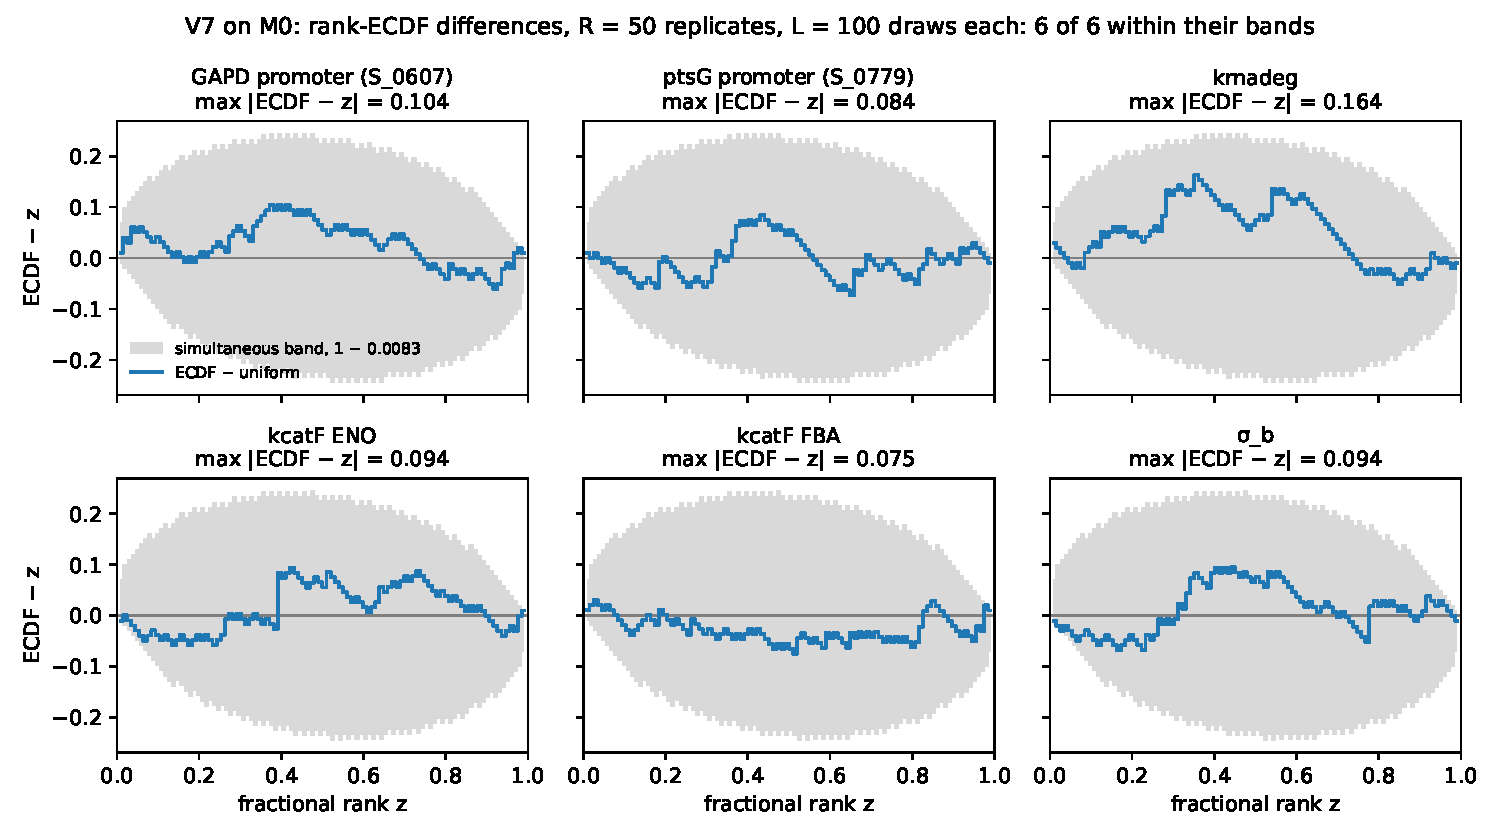
\includegraphics[width=0.48\textwidth]{f8_rank_ecdf.pdf}\hfill
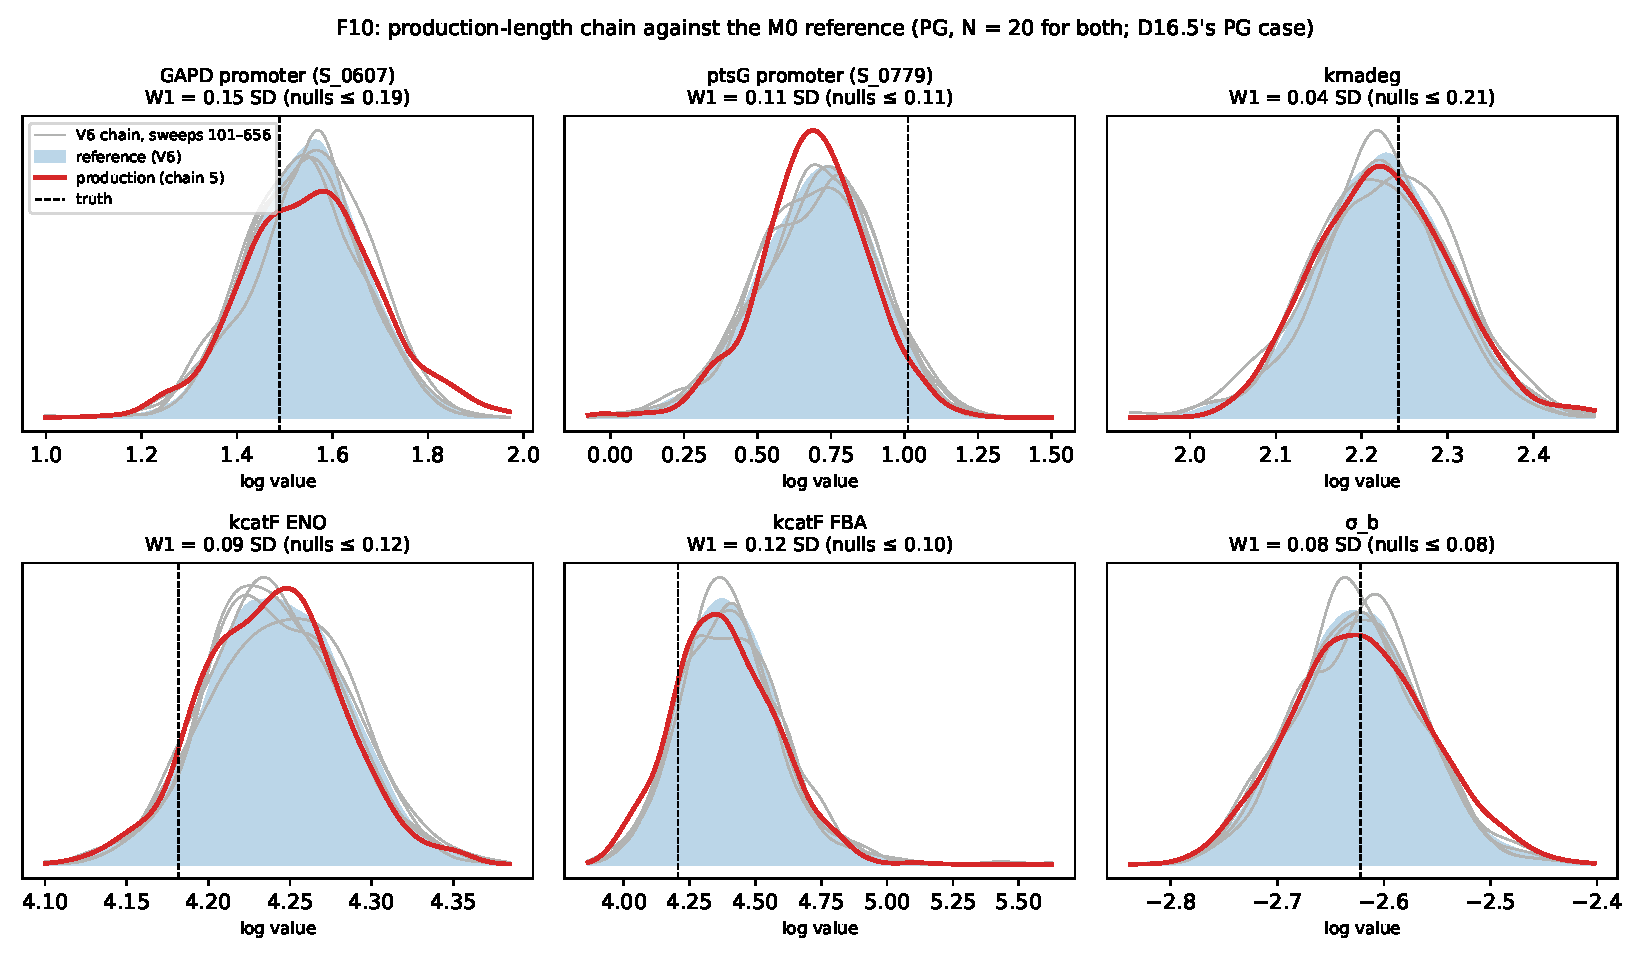
\includegraphics[width=0.48\textwidth]{f10_marginals.pdf}
\caption{\textbf{The exact sampler on M0.} (a) Rank-ECDF of the truth over
\pn{vseven.R} prior-drawn datasets, against simultaneous 95\% bands. (b) Marginal
posteriors from a production-length chain against the reference.
\placeholder{Restyle both panels to one figure with shared fonts; label panels.}}
\label{fig:calibration}
\end{figure*}

\subsection{The cost of the formalism swap is declared and measured}
\label{sec:jensen}

The mean-field swap replaces the stochastic gene expression with its mean. The
means of transcripts and proteins are exact, but metabolism is nonlinear. A
metabolism fed the mean drain differs from the mean over cells of metabolisms fed
their own drains. The difference is a Jensen gap.

\paragraph{The cause.} The gap is largest for GTP, where the mean field sits
\pn{jg.gtplo}--\pn{jg.gtphi}\% below the population mean. We traced it to
cell-to-cell variation in the drains. When every cell receives the mean field's
drains, the mean over cells equals the mean field to three significant figures. We
ruled out the enzyme counts, the per-cell feedback and the clip at zero as causes of
the GTP gap. A likely mechanism, which we have not tested, is that only saturable
enzymes regenerate GTP. Then cells that spend more GTP lose more of it than cells that
spend less gain back, and the population mean sits above GTP at the mean spend.

\paragraph{The correction.} We treat the gap as a declared reduction and correct it
with an offset $\delta$, the log difference between the mean of a reference
ensemble and the mean field at one reference parameter set. Our reference is the
most detailed composition we have, the exact hybrid, and not the truth about the
cell. We report the gap with a goodness check and with the parameter bias it
implies, and we do not use it as a stop.
\begin{itemize}
  \item Without $\delta$, the gap would move the transcript decay rate by
  \pn{jg.biaslo}--\pn{jg.biashi} posterior standard deviations.
  \item With $\delta$, the remaining bias is within about one standard deviation.
  \item The goodness check as first written fails a description known to be correct
  in about half of all cases: a correct description passes only
  \pn{jg.kgnulllo}--\pn{jg.kgnullhi}\% of the time. We therefore compare the check
  with its own null distribution. With $\delta$, the mean field falls inside the
  null's 95\% range at \pn{jg.deltain} targets, against \pn{jg.mfin} without
  $\delta$.
\end{itemize}

\paragraph{The mean-field model is the limit of the hybrid.} The hybrid exchanges
state every second. As this step shrinks, the hybrid's mean converges to the
one-ODE mean-field model. At the zero-step limit the two agree to
\pn{rii.maxdelta} in log concentration at all five test parameter sets. One
mean-field solve takes \pn{rii.mzero}\,s on M0 and \pn{rii.corealo}--\pn{rii.coreahi}\,s
on the full reduced model.

\placeholder{AV6 (B7) decides whether the remaining gap moves the posterior. Add one
sentence with the answer.}

\subsection{The approximate posterior agrees with the exact one on M0}
\label{sec:approx}

\placeholder{B7 / AV6, not run. Refit the \pn{vseven.R} V7 datasets with the
approximate route. Report: overlaid marginals and the ptsG--ENO contour against the
exact posterior; rank-ECDF of the approximate route; cost per posterior against
\pn{ften.cpuh} CPU-hours. Gate: M0 carries a metabolite $\to$ ptsG signal (linearised
ratio \pn{info.mzeroptsg} against a noise bracket of \pn{info.mzerobracket}; met).}

\begin{figure*}[t]
\centering
\placeholderfig{0.9\textwidth}{5cm}{Figure 5: approximate against exact on M0.
Overlaid marginals, the ptsG--ENO contour, rank-ECDF, and a cost bar. Not run (B7).}
\caption{\textbf{Approximate against exact.} \placeholder{Caption.}}
\label{fig:approx}
\end{figure*}

\subsection{Inference on the full reduced model}
\label{sec:fullscale}

\placeholder{B8 / AV7, not run; needs the cap reopened (O1). Calibration over
$\ge 200$ injections on the full reduced model. Posterior widths against the
linearised information bound for the six D11 targets. The F6 table: transcripts
only, metabolites only, both. Target from the bound: ptsG under metabolites only at
\pn{info.ptsg} of its prior SD (bracket \pn{info.ptsgbracket}); ENO at \pn{info.eno}
(bracket \pn{info.enobracket}).}

\begin{figure}[t]
\centering
\placeholderfig{\columnwidth}{5cm}{Figure 6 (F6): posterior/prior SD per target under
three data regimes, with the information bound drawn on. Not run (B8).}
\caption{\textbf{What each data stream informs.} \placeholder{Caption.}}
\label{fig:f6}
\end{figure}

\subsection{The uncertainty budget of a prediction}
\label{sec:budget}

\placeholder{Not built (outline §6). Draw the inferred parameters from the posterior
and all others from their priors; run the coupled model; split the variance of an
unobserved quantity (fractional growth, lactate export, or how often GTP empties)
into: inferred parameters, parameters left at their priors, and intrinsic noise.
Report the split with asserted prior widths halved and doubled. Target sentence:
``x\% of the uncertainty in this prediction comes from parameters that no
measurement supports.'' About 50 CPU-h on M0.}

\begin{figure}[t]
\centering
\placeholderfig{\columnwidth}{4.5cm}{Figure 7: the uncertainty budget of one
prediction. Not built.}
\caption{\textbf{Where the uncertainty of a prediction comes from.}
\placeholder{Caption.}}
\label{fig:budget}
\end{figure}

\subsection{Cost}
\label{sec:cost}

\Cref{tab:cost} gives the cost of one posterior by each route. An exact posterior on
the full reduced model is projected at about \pn{cost.fullscale} CPU-hours, above
our bound of \pn{cost.kone} CPU-hours per posterior. Exact inference therefore
stops at M0. The cost is the number of simulations, not the time of one. One cycle
of the full reduced model takes \pn{model.cyclewall}\,s, and a fast
implementation of the full \syn{} model is the subject of a companion paper
\citep{kimpson2026whole}.

\begin{table}[t]
\caption{CPU-hours per posterior.}
\label{tab:cost}
\centering
\small
\begin{tabular}{@{}lcc@{}}
\toprule
Route & M0 & Reduced model \\
\midrule
Exact, reference & \pn{vsix.cpuh} & --- \\
Exact, production & \pn{ften.cpuh} & $\sim$\pn{cost.fullscale} (projected) \\
Approximate & \placeholder{B7} & \placeholder{B8} \\
\bottomrule
\end{tabular}
\end{table}
